%Chapter 5

\renewcommand{\thechapter}{5}

%TODO: Add better title
\chapter{System Implementation}
\label{ch:system_implementation}

Given its grandiose title, it may seem that the engineering behind the development of a planetary scale data storage system would require thousands of man-hours of professional software engineers and a highly structured development process.
In fact, this is not necessarily the case for two reasons.
First, data systems benefit from an existing global network topology and commercial frameworks for deploying applications.
This means that both the foundation and motivation for creating large geo-replicated systems exists, as described in Chapter~\ref{ch:architecture}.
Second, like the Internet, complex global systems emerge through the composition of many simpler components following straight forward rules~\cite{internet}.
Instead of architecting a monolithic system, the design process is decomposed to reasoning about the behavior of single processes.

Fundamentally, each process in our system is an independent actor~\cite{actors,scala_actors,orleans} with storage, memory, and compute resources.
The primary purpose of an actor is to receive and respond to messages (events) from other actors by modifying the actor's internal state, creating new actors, or sending messages to other actors~\cite{hewitt_actors}.
The behavior of an actor depends solely on the order of messages received, making them an ideal model for programming consistency protocols.
A system is therefore composed of actors, and reasoning about the global behavior of the system requires only a description of the interactions that different actors in the system have.

The actor model allows us to decouple consistency behavior from application behavior.
Consistency behavior is defined in the messaging between actors, for example actors participating in hierarchical consensus provide consistency by voting for a leader and correctly committing commands from the leader based on majority votes.
Application behavior is defined by the internal state of the actor, for example the maintenance of a versioned key-value store.
We use this decoupling to construct two principle applications from our consistency-centric model: a key-value database and a file system, all distributed geographically.

In this chapter we will describe the details of our implementation.
First, we will describe the base requirements for all replicas, along with our assumptions concerning communication, security, processing and data storage.
We will also outline the details of our implementation of the consistency protocols described in previous chapters.
Both HC and federated consistency are based on object stores that can be sharded and managed independently, therefore we will principally describe operations in terms of a key/value store.
Finally we will describe the details of the applications we built on top of our consistency protocols and the base object store.

\section{Replicas}
\label{ch05_replicas}

The primary actor in our system is the \emph{replica}.
Replicas are independent processes that maintains a portion of the objects stored as well as a \emph{view} of the state of the entire system.
Each replica implements a shared-nothing architecture~\cite{shared_nothing} such that each replica has its own memory and disk space.
For practical purposes of fault tolerance, we generally assume that there is a one-to-one relationship between a replica and a disk so that a disk failure means only a single replica failure.
Replicas must be able to communicate with one another and may also \emph{serve} requests from clients.
By default we assume that all replicas in the system are addressable and that both clients and peers can send messages to all replicas in the network, barring failures.

A system is composed of multiple communicating replicas and is defined by the behavior the replicas.
For example, a totally replicated system is one where each replica stores a complete copy of all objects as in the primary-backup approach~\cite{primary_backup}, whereas a partially replicated system ensures durability such that multiple replicas store the same object but not all replicas store all objects as in the Google File System (GFS)~\cite{gfs}.
At the scale of a multi-region, globally deployed system, we assume that total replication is impractical and primarily consider the partial replication case.
However, we also assume that replicas maintain a view of the entire system, that is meta-data about the location and provenance of all objects, so as to direct client requests to the appropriate replica to serve requests.

Replicas primarily cache their object stores in memory to improve performance.
If a replica fails it can be brought up to date by a peer replica through either consistency protocol.
Durable storage is written to asynchronously, to minimize the amount of recovery time required for a replica.
Our implementation can use multiple backend stores, writing pages and logs to disk, or using embedded key/value stores such as LevelDB~\cite{leveldb}, BadgerDB~\cite{badgerdb}, or PebblesDB~\cite{pebblesdb}.
These databases use the ext4 file system, though in the future we hope to investigate the use of a tree-based file system to more directly optimize disk usage~\cite{btrfs}.

We assume that replicas reside on trusted hosts with reliable communication and that failures are non-byzantine~\cite{byzantine-generals,byzantine_fault_tolerance}.
However, we do expect security to be a default component of a real-world implementation, particularly as many communication links travel across the Internet.
Communication should be secured and authenticated with transport layer security (TLS)~\cite{tlsv1,tlsv2}.
TLS requires that each replica maintains a certificate and public key encryption to secure communications~\cite{rsa} and if each replica has its own certificate, then TLS can also be used to authenticate valid peers based on a central authority's shared certificate~\cite{tls_authentication}.
We also assume that data stored on disk should be encrypted.
We prefer per-replica encryption to ensure that data is loaded and stored from an in-memory cache as quickly as possible though we recognize that some applications require per-user encryption; it is beyond the scope of our system to provide it.

\begin{figure}
    \begin{center}
        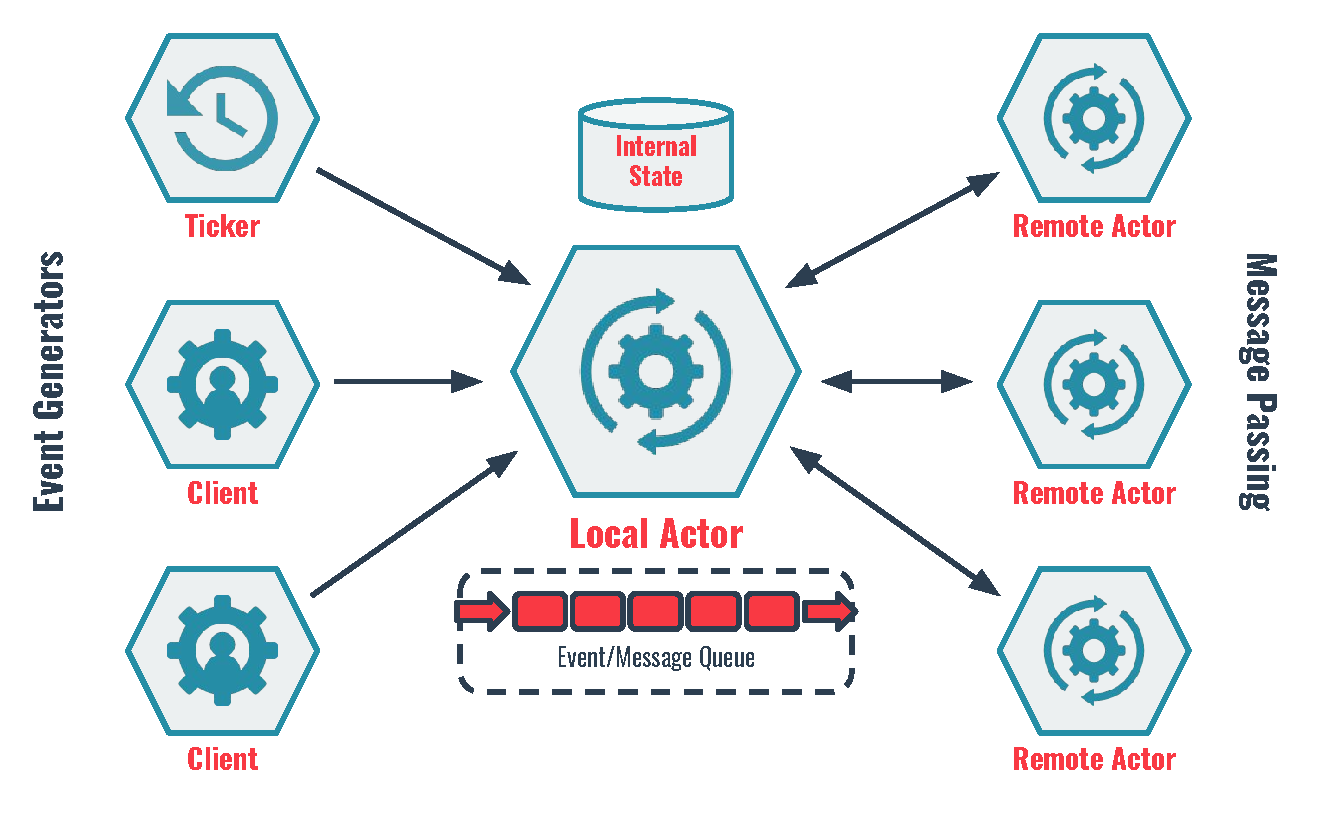
\includegraphics[width=5in]{figures/ch05_actor_model.pdf}
    \end{center}
    \renewcommand{\baselinestretch}{1}
    \small\normalsize

    \begin{quote}
        \caption[Replica Actor Model]{Each replica is an actor that maintains an internal state that is modified by processing messages from other actors. Implemented in the Go programming language, each event is serialized by a single message channel ensuring that the state is modified correctly.}
        \label{fig:ch05_actor_model}
    \end{quote}
\end{figure}
\renewcommand{\baselinestretch}{2}
\small\normalsize

All replicas are implemented in Go~\cite{golang}, a systems programming language that provides concurrency through communication channels~\cite{csp}.
Each replica implements a primary event loop as a single channel to ensure that all events and messages are serialized in a single order as shown in Figure~\ref{fig:ch05_actor_model}.
This prevents the need to use multiple expensive mutexes to synchronize the behavior of multiple threads and allows us to more easily reason about the operation of the system.
Communications are implemented using gRPC~\cite{grpc}, an HTTP communication protocol that serializes messages in protocol buffers format~\cite{protocol_buffers} which allows clients to be implemented in multiple programming languages.
The gRPC server accepts new requests each in an independent thread.
Clients are handled using unary RPC requests, but to improve communication performance between replicas we use bilateral streaming.
Bilateral streaming also guarantees that if online, replicas will receive messages in the order they are sent.
Each message is pushed through the primary event channel, then responded to using a callback channel.
Other threads include timers and monitoring routines that are also synchronized through the main event channel.

We've principally implemented two types of replicas with two different consistency protocols.
Alia~\cite{alia} replicas implement hierarchical consensus based on our implementation of the Raft protocol~\cite{alia_raft}.
Honu~\cite{honu} replicas implement eventual consistency using bilateral anti-entropy synchronization.
Both Alia and Honu implement an object store such that objects are described by unique keys, and each update to the object creates a new version.
The key/value nature of our implementation allows the namespace and object data to be sharded and partially replicated across all replicas, therefore the key/value database described in \S~\ref{ch05_key_value_db} is the base application for all of our applications.
The details of each replica type follows.

\subsection{Alia}
\label{ch05_alia}

Alia replicas implement hierarchical consensus.
Each replica process runs multiple instantiations of a modified Raft protocol in independent threads as shown in Figure~\ref{fig:ch05_hc_actor_model}.
Every replica must run one instantiation of the \textit{root consensus protocol}.
Replicas may also run one or more instantiations of the \textit{commit consensus protocol} if they are assigned to a subquorum.
It is imperative that our implementation runs a single process with multiple threads, if the replica crashes it must not participate in either root consensus or subquorum consensus.
This is further ensured by a main thread, the ``Alia Actor'' which acts as the gRPC server dispatching messages to the appropriate quorum.
The Alia Actor also handles process-level events like metrics gathering, operating system signals, and maintaining connections to remote peers.
Although this does incur some overhead as shown in Figure~\ref{fig:ch05_alia_raft_overhead}, it is far outweighed by the benefits of scaling consensus across multiple subquorums.

\begin{figure}
    \begin{center}
        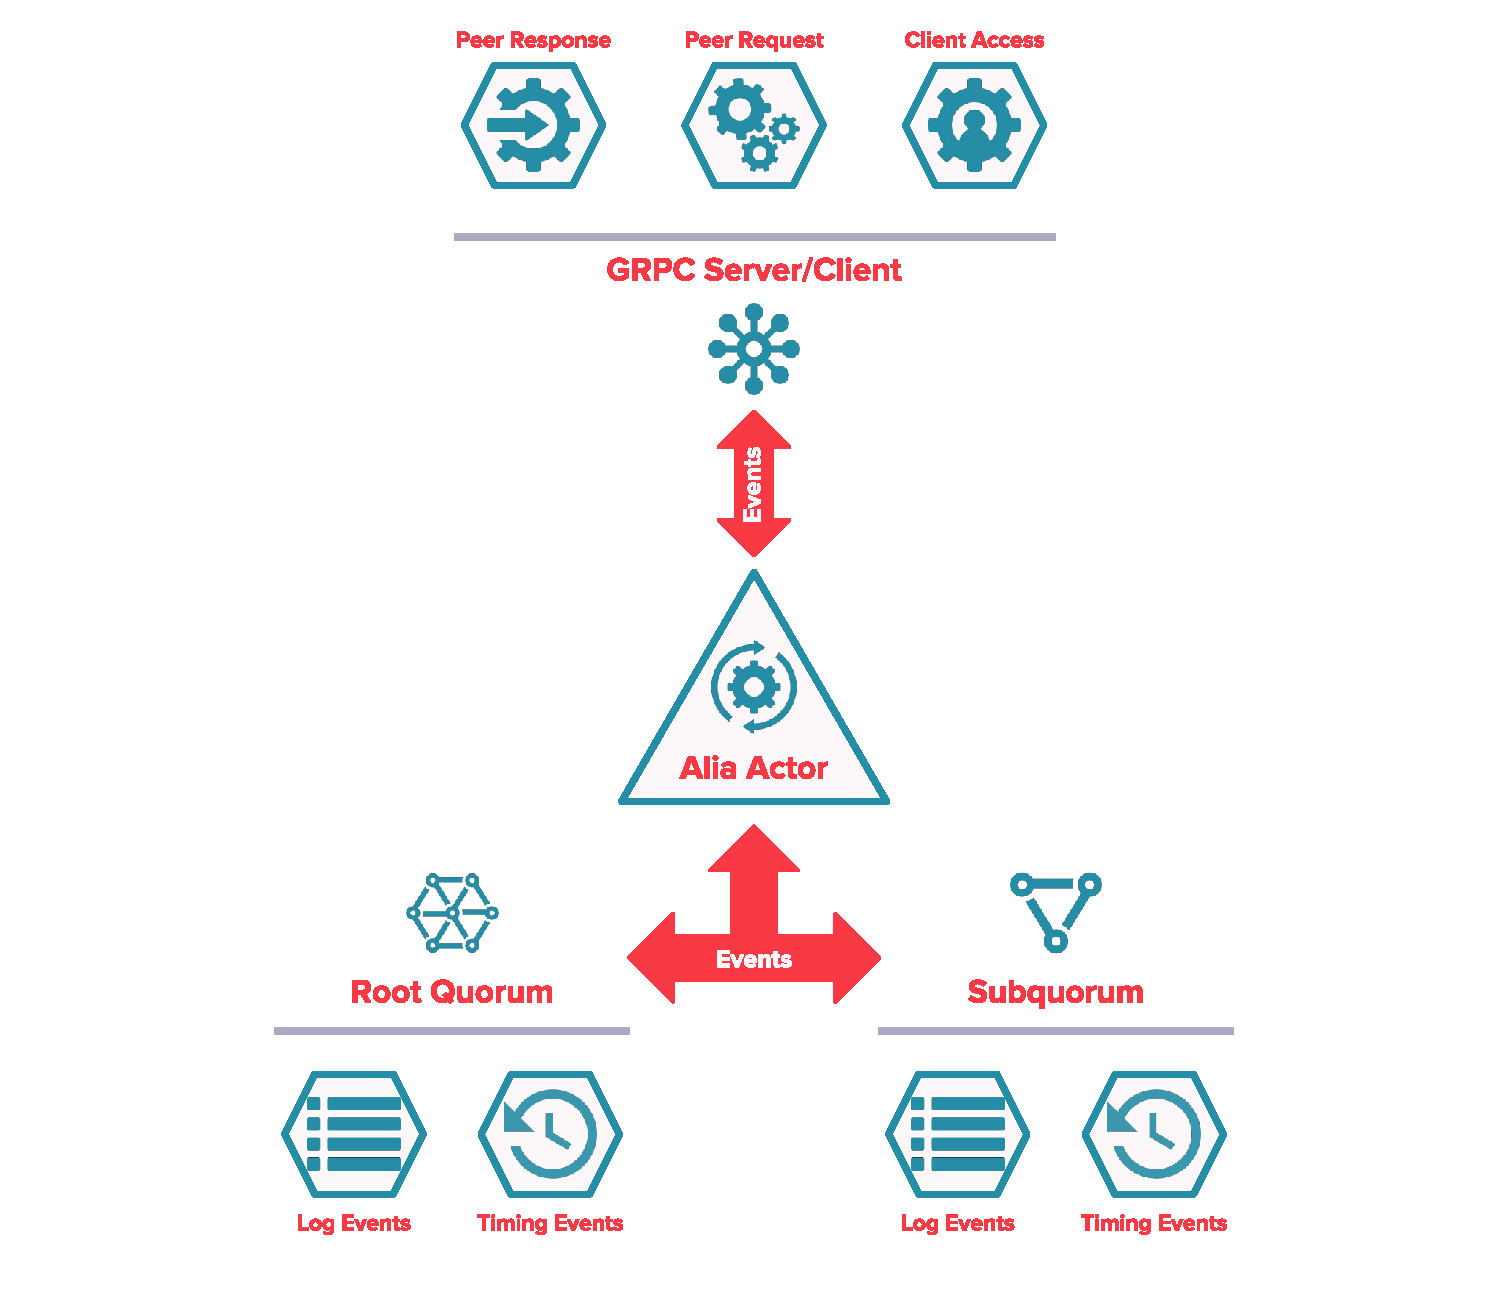
\includegraphics[width=5in]{figures/ch05_hc_actor_model.pdf}
    \end{center}
    \renewcommand{\baselinestretch}{1}
    \small\normalsize

    \begin{quote}
        \caption[Alia Actor Model]{The Alia actor model model is composed of at least three primary actors: the root quorum actor, a subquorum actor, and the main actor that dispatches messages to each subquorum. Other minor actors such as client requests threads and timing events dispatch their messages directly to their associated actors.}
        \label{fig:ch05_hc_actor_model}
    \end{quote}
\end{figure}
\renewcommand{\baselinestretch}{2}
\small\normalsize

\begin{figure}
    \begin{center}
        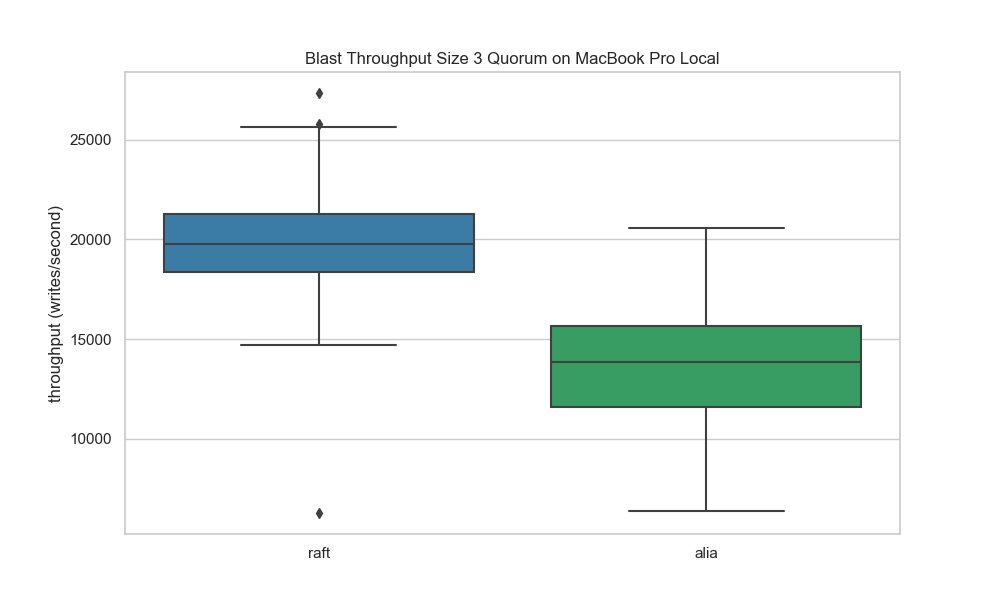
\includegraphics[width=5in]{figures/ch05_alia_raft_overhead.png}
    \end{center}
    \renewcommand{\baselinestretch}{1}
    \small\normalsize

    \begin{quote}
        \caption[Overhead of Root Consensus]{Running multiple consensus instances in the same process does incur some overhead over a single consensus algorithm, but this overhead is minimal when global throughput is considered.}
        \label{fig:ch05_alia_raft_overhead}
    \end{quote}
\end{figure}
\renewcommand{\baselinestretch}{2}
\small\normalsize

All actors, but especially the quorum actors implement an event loop that responds to timing events, client requests, and messages from peers.
Events may cause the replica to change state, modify a command log, broadcast
messages to peers, modify the key-value store, or respond to a client.
Event handlers need to aggressively lock shared state for correctness because Golang and gRPC make extensive use of multi-threading.
The balance between correctness and concurrency-driven performance leads to
increasing complexity and tighter coupling between components, one that
foreshadows extra-process consistency concerns that have been noted in other
work~\cite{paxos_live,raft,raft_students_guide}.
Our implementation handles this in two ways.
First, gRPC bidirectional streaming ensures that if a remote peer is online, replies to messages between two peers are delivered in order in which they were sent.
Second, each actor uses a single event channel to serialize the sequence of events being handled.
This significantly reduces the number of mutexes in our system to basically zero.

Both the root quorum and subquorums in our implementation use timing parameters to detect when changes need to be made to their state.
Timing parameters depend on the network environment since timers are often reset when messages arrive.
For example, both the obligations timeout and the election timeout are reset when a heartbeat message is received from the root leader and quorum leader respectively.
This means timeouts must be much greater than the average time to broadcast and receive responses, and much less than the mean time between failures~\cite{raft,etcd_raft,oliveira_evaluating_2016}.
If this requirement is not met, the system may simply become unavailable as it cannot recover from leadership failures.

As described in \S~\ref{ch04_timing}, we use a tick parameter, $T$ that is a function of the mean network latency ($\lambda_{\mu}$) to describe timing events.
In a stable network environment, Howard et al~\cite{raft_refloated} proposes  $T=\lambda_{\mu}+2\lambda_{\sigma}$ to maximize leader availability.
Other more conservative implementations such as etcd~\cite{etcd_raft} use $T=10\lambda_\mu$ or allow the user to specifically configure the tick.
In both cases, standard Raft generally defines the heartbeat interval as $\frac{T}{2}$, and the election timeout as the interval $U(T,2T)$.
Our implementation allows multiple functions for defining $T$, but parameterizes the timing intervals as shown in Table~\ref{tab:ticks}.

\renewcommand{\baselinestretch}{1}
\small\normalsize
 \begin{table}[t!]
\caption[Parameterized Timeouts of HC Implementation]{Timing intervals play a significant role in determining replica action in our implementation of Raft. This table shows the relationship between timing intervals using a tick parameter, $T$ ($T=45 ms$ for our experiments on Amazon EC2).}
\begin{center}
\begin{tabular}{l|c|l}
\hline
Timeout & Interval & Action \\
\hline \hline
\texttt{Heartbeat} & $1T$ & subquorum leader broadcasts heartbeat\\
\texttt{Election} & $U(2T,4T)$ & become subquorum candidate \\
\texttt{AntiEntropy} & $4T$ & synchronize with non-quorum peer \\ \hline
\texttt{RootHeartbeat} & $10T$ & root leader broadcasts heartbeat \\
\texttt{RootElection} & $U(20T,40T)$ & become root candidate \\ \hline
\texttt{Obligations} & $10T$ & root leader may reconfigure \\
\texttt{Beacon} & $U(100T,200T)$ & send summary stats to leader \\
\hline
\end{tabular}
\end{center}
\label{tab:ticks}
\end{table}
 \renewcommand{\baselinestretch}{2}
\small\normalsize

\textbf{Changes to base Raft:} In addition to major changes, such allowing replicas to be part of multiple quorums simultaneously, we also made many smaller changes that had pervasive effects.
One change was including the \textit{epoch} number alongside the term in all log entries.
The epoch is evaluated for invariants such as whether or not a replica can append an entry or if a log is as up to date as a remote log.

Vote delegation requires changes to vote counting.
Since our root quorum membership actually consists of the entire system, all replicas are messaged during root events.
All replicas reply, though most with a ``zero votes'' acknowledgment.
The root uses observed vote distributions to inform the ordering of future consensus messages (sending requests first to replicas with votes to cast), and uses timeouts to move non-responsive replicas into ``hot spares'' status.

One major change we made to dramatically improve performance is to aggregate \texttt{AppendEntries} requests to serve multiple client requests in a single round.
Such requests are collected while an outstanding commit round is ongoing, then sent together when that round completes.
Because all requests are sent through a single channel, we simply read off the channel until it is empty or another event type has occurred before creating a multi-entry append and sending it.
The root quorum also aggregates all requests within a minimum interval into a single new epoch-change/reconfiguration operation to minimize disruption.

Commits are observed by the leader once a majority of replicas respond positively.
Other replicas learn about the commit only on the next message or heartbeat.
Root epoch changes and heartbeats are designed to be rare, meaning that epoch change commits are not seen promptly.
We modified the root protocol to inform subquorums of the change by sending an additional heartbeat immediately after it observes a commit.
Root heartbeat messages also serve to notify the network about events that do not require an epoch change, such as the election of a new subquorum leader or bringing a failed node back online.

Replicas may be part of both a subquorum and the root quorum, and across epoch boundaries may be part of multiple subquorums.
In principle, a high performance replica may participate in any number of subquorums.
We therefore allow replicas to accommodate multiple distinct logs with different access characteristics.
Peers that are either slow or with unsteady connectivity are occasionally left behind at subquorum leader or epoch changes.
Root heartbeats containing the current system configuration are broadcast to all replicas and serve to bring them up to date.

Finally, consensus protocols often synchronously write state to disk before responding to remote requests.
This allows replicas that merely crash to reboot and rejoin the ongoing computation after recovering state from disk.
Otherwise, these replicas need to go through heavyweight leave-and-rejoin handshakes.
Our system avoids these synchronous writes by allowing epochs to re-join a subquorum at the next epoch change without any saved state, avoiding these handshakes altogether.

\subsection{Honu}
\label{ch05_honu}

Honu replicas implement our eventual consistency fog with anti-entropy synchronization and are considerably simpler than their Alia counterparts.
Each Honu replica maintains an in-memory cache of key-value pairs.
To reduce contention and respond to requests as quickly as possible, the in-memory cache is itself sharded and uses a simple hash of the key to determine object placement.
Each shard is then protected by a read/write mutex.
Reads are immediately returned from the in-memory cache.

Writes are applied to the in-memory store asynchronously.
When a write is requested by the client, the update is first appended to a log on disk before responding successfully to the client.
A background thread consumes the log, applying each write first to an embedded key/value store on disk, then to the in-memory cache.
This ensures that all reads return writes that have been saved to durable storage but increases the likelihood of stale reads: our model optimizes for high-throughput writes and rarer reads.

As the background process applies writes, it updates the version of the object and links the version to its parent version.
Object versions are defined by conflict-free version numbers~\cite{version_conflict_detection,version_vectors} comprised of three components: a precedence ID, a monotonically increasing scalar, and the ``forte'' number.
The precedence ID must be unique per replica and can either be configured or based on the network address of the replica such as a GUID.
Both the scalar and forte component can optionally be across all objects (so as to compare if a write to object A is later than a write to object B) or on a per-object basis depending on the requirements of the system.
Versions are compared by first comparing the forte numbers, then the scalar component, then in the case of ties, the precedence ids.

On a periodic interval, Honu replicas perform background anti-entropy synchronization.
On each interval, the replica selects a remote peer using a scheme such as those described in Chapters~\ref{ch:federated_consistency} and~\ref{ch:adaptive_consistency} or by simply using uniform random selection.
The latest local versions of each object in the in-memory cache are collected as quickly as possible by a parallel read of each in-memory shard that returns a per-shard mapping of key to version (each shard is read locked for the duration of the read).
Once the versions are collected, they are assembled into a binary Merkle tree~\cite{merkle_tree} by lexicographically sorting the keys whose data is their version number.
This tree is cached in case the local replica is chosen for synchronization by another replica.
The version tree (or array in simpler implementations) is then sent to the selected peer.

When the remote peer receives the pull request, it compares the arriving version tree with its local tree to quickly determine which objects if any have been updated.
The remote peer returns objects for all versions that the remote peer has that are later than the version of the object described by the initiating peer.
Additionally it sends the initiating peer a push request for all versions that are earlier on the remote peer, updating both the scalar and forte components as needed.
The initiating peer concludes the synchronization by applying the later versions to its store, updating its scalar and forte components, then sending back the requested objects to the remote replica.

\section{Applications}
\label{ch05_applications}

We target two primary applications: a globally distributed key/value database and file system.
Both Alia and Honu manage a key/value object store by applying operations asynchronously from a log of command operations.
Both of these object stores are native for different reasons.
Alia replicas require a key/value object store so that the namespace can be appropriately sharded to individual subquorums.
Subquorums then commit entries to a log, which are then applied to an in-memory cache for quick read accesses and to an embedded key/value database for durable storage and to snapshot and archive the log files.
Honu replicas manage a key/value object store to minimize contention when writing to an in memory cache and to provide a framework for anti-entropy synchronization.
Updates to the cache are also implemented asynchronously from a log, but consistency is relaxed so that no coordination is required and to return to the client as fast as possible.

\begin{figure}
    \begin{center}
        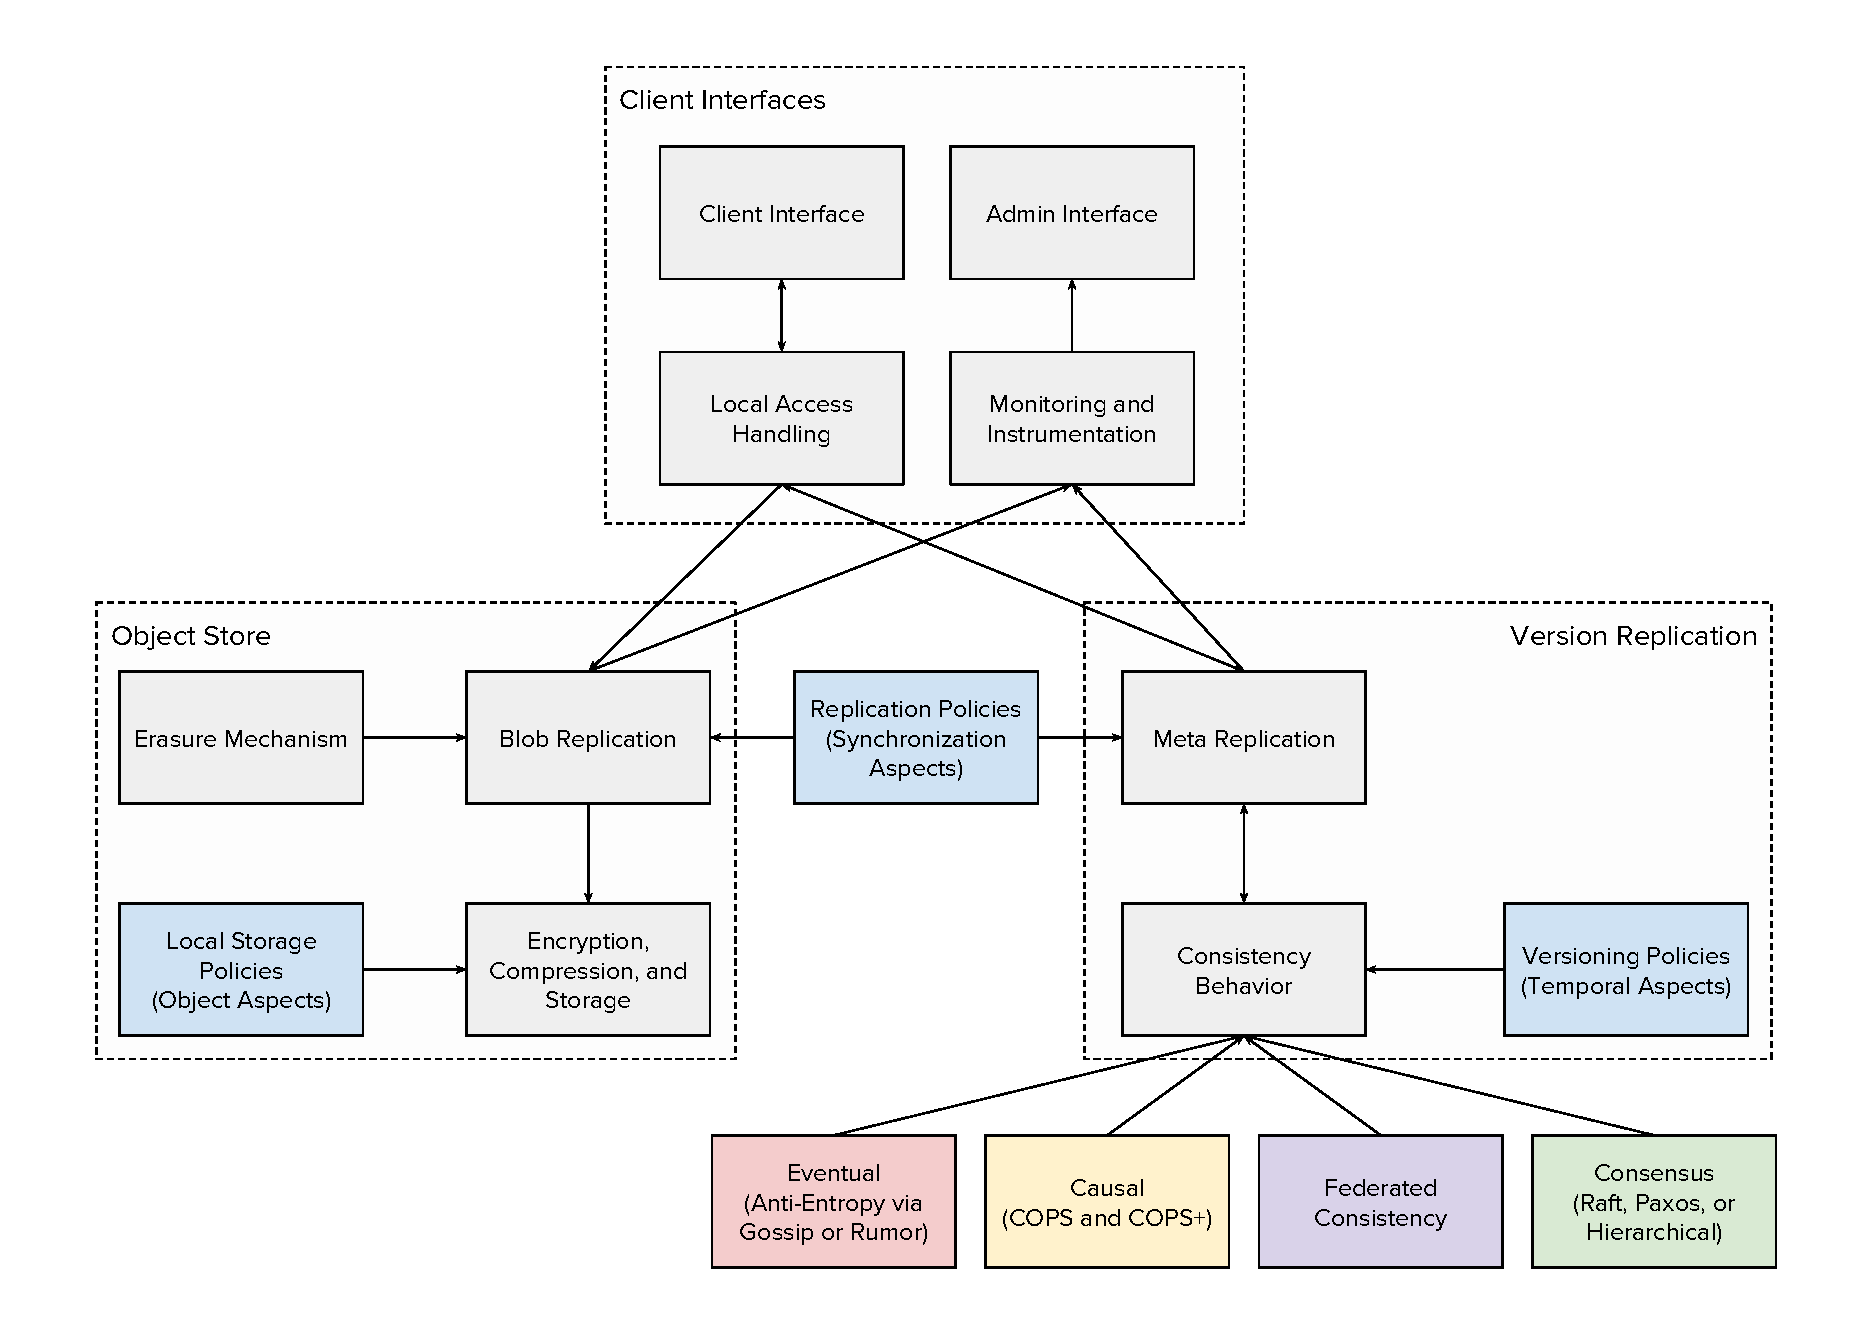
\includegraphics[width=\linewidth]{figures/ch05_fluidfs_components.pdf}
    \end{center}
    \renewcommand{\baselinestretch}{1}
    \small\normalsize

    \begin{quote}
        \caption[Application Component Model]{This architecture provides a general component model for consistency-centric applications. Object blobs and version metadata are replicated separately to allow partial replication of data but a full view of the current state of the system. Only version replication requires consistency semantics, therefore our federated and hierarchical consensus models only deal with metadata commands.}
        \label{fig:ch05_fluidfs_components}
    \end{quote}
\end{figure}
\renewcommand{\baselinestretch}{2}
\small\normalsize

We decompose the storage requirements for each application into three aspects as shown in our general component model in Figure~\ref{fig:ch05_fluidfs_components}.
\emph{Object aspects} describe the local storage policies of blobs of data representing the objects.
These aspects inform the system of the durability of the object, e.g. to how many disks/zones the data is replicated as well as other policies such as erasure, compression, or encryption.
\emph{Temporal aspects} describe how different versions of data in the system are managed, e.g. how many versions to keep or how a user goes back in time to find earlier or later versions of a file.
Versions also define the external view of the system, therefore only version information need be consistently replicated.
Finally, \emph{Synchronization aspects} define how both blobs and meta data are replicated across the system, and have been the primary subject of this chapter.

We point out these aspects primarily to identify them as belonging to the application layer rather than to our data model.
Multiple policies across one or more of these aspects can be easily implemented in an application without requiring a change to hierarchical consensus, federated consistency, or adaptive consistency.
In this section we will describe some of the choices we have made in our target applications.

\subsection{Key/Value Database}
\label{ch05_key_value_db}

A key/value database is a natural extension to our proposed data model.
Both Alia and Honu replicas operation on a key based object model such that keys are structs that contain a unique name, version, and parent version and values are blobs of binary data.
To generalize this to a key/value database, the application must map arbitrary keys (which can be arrays of bytes or strings) to arbitrary objects (which might also contain type information).
We accomplish this by maintaining an additional data structure that maps application keys to their object/version key as well as type information.
Values are then serialized into blobs either by marshaling them as JSON data or in Protocol Buffers format.

Clients can make \texttt{Get}, \texttt{Put}, and \texttt{Del} requests by default.
\texttt{Get} requests return the latest version of the object for a user specified key according to the read policy of the replica.
Alia replicas forward the request to the leader of the subquorum managing the tag that contains the key by inspecting the configuration defined by a prefix trie that maps keys to subquorums (responding to a request requires at most two redirects).
The leader then returns the latest committed value of the key.
Honu replicas simply return the latest value of the object as found in their local cache.
\texttt{Put} requests are similarly forwarded to the leader of the subquorum, which then initiates a consensus round and returns the version of the update to the client when the update is committed.
Honu replicas similarly update their local version then return to the client when the update has been written to stable storage.
If the client requires the new version, Honu may block until the update is applied.

\texttt{Del} requests are considered updates, but do not actually erase data.
Instead, a tombstone version is written to the object store with no associated data.
On \texttt{Get}, if a tombstone version is encountered, a not found error is returned to the client; on \texttt{Put} the version history is continued such that the parent version is the tombstone version -- applications can then decide whether or not to allow users to go back in time to deleted versions, or to use tombstone versions as checkpoints to clean up data and reduce storage overhead.
Other types of accesses are also possible for other data types, for example an array datatype might allow \texttt{Append} accesses or a set datatype,  \texttt{Union} or \texttt{Intersect} operations.
In these cases, the operation is treated as a \texttt{Get} then \texttt{Put} using the semantics described above.


\subsection{File System}
\label{ch05_file_system}

Our file system, called FlowFS, like many modern file systems, decouples meta-data~\emph{recipes}~\cite{casper,gfs,hadoop_hdfs,pvfs,globalfs} from file data storage.
Meta-data includes an ordered list of \emph{blobs}, which are opaque binary chunks.
When a file is closed after editing, the data associated with the file is \emph{chunked} into a series of variable-length blobs~\cite{lbfs}, identified by a hashing function applied to the data~\cite{rabin_karp,rabin_fingerprint}.
Since blobs are effectively immutable~\cite{immutability_changes_everything}, or tamper-evident, (blobs are named by hashes of their contents), we assert that consistent meta-data replication can be decoupled from blob replication.
Accesses to file system meta-data becomes the primary consistency operations.
For simplicity we describe our file system using HC.

FlowFS aggregates individual accesses into \textit{Close-To-Open} (CTO)~\cite{afs,coda,orifs,sundr,globalfs} consistency such that read and write accesses are ``whole file'' \cite{lbfs}.
A file read (``open'') is guaranteed to see data written by the latest write (``close'').
This approach satisfies two of the major tenets of session consistency: \texttt{read-your-writes} and \texttt{monotonic-writes}, but not \texttt{writes-follow-reads}~\cite{bermbach_consistency_2013,anti_entropy,eventual_consistency}.
These guarantees are necessary to provide file system semantics and are enabled by local cacheing.
Intermediate sync and flush operations are written to disk and replication only occurs when a file is closed.
Stronger consistency is possible if clients are allowed to request leases on files, though this has implications for epoch transition that must be more fully considered.

The file system is defined as a hierarchical namespace, which is itself defined as an object store with complex keys, similar to Amazon S3~\cite{bermbach_eventual_2011}.
In principle there are two types of objects: directories and files, however, to implement sharding across multiple subquorums, in reality there are files and containers, directories that contain files and are specifically managed by a subquorum.
This is necessary otherwise adding a file to a directory would require updating the versions of all containers up to the root, which would require coordination between all subquorums.
Instead, the namespace is partitioned by a prefix, which defines a container. For example, \texttt{alia://us-east-1/edu.umd.cs/~bengfort/*} would indicate that a subquorum is responsible for all objects under the described prefix.
Read operations on non-container prefixes are still possible, but rather than returning data, would instead return the subquorums that manage that space.

When a file is closed after editing the version and data are prepared for replication.
Version information is updated as in the key/value database and replicated using the consistency policy of the replica.
The data associated with the file is chunked into a series of unique, variable-length blobs that are stored in a directory structure based on the blobs hash (thereby allowing easy computation of a modified Merkle tree structure for anti-entropy replication).
On read, the replica demand-fetches the blobs to return data to the client.
Techniques like hoarding \cite{kuenning_automated_1997} and TCP layer replication \cite{venkataramani_operating_2002} can improve blob replication, optimistically colocating blobs with likely read accesses. However, if a blob is not available locally a remote access to a storage device with the blob is all that is required.

\begin{figure}
    \begin{center}
        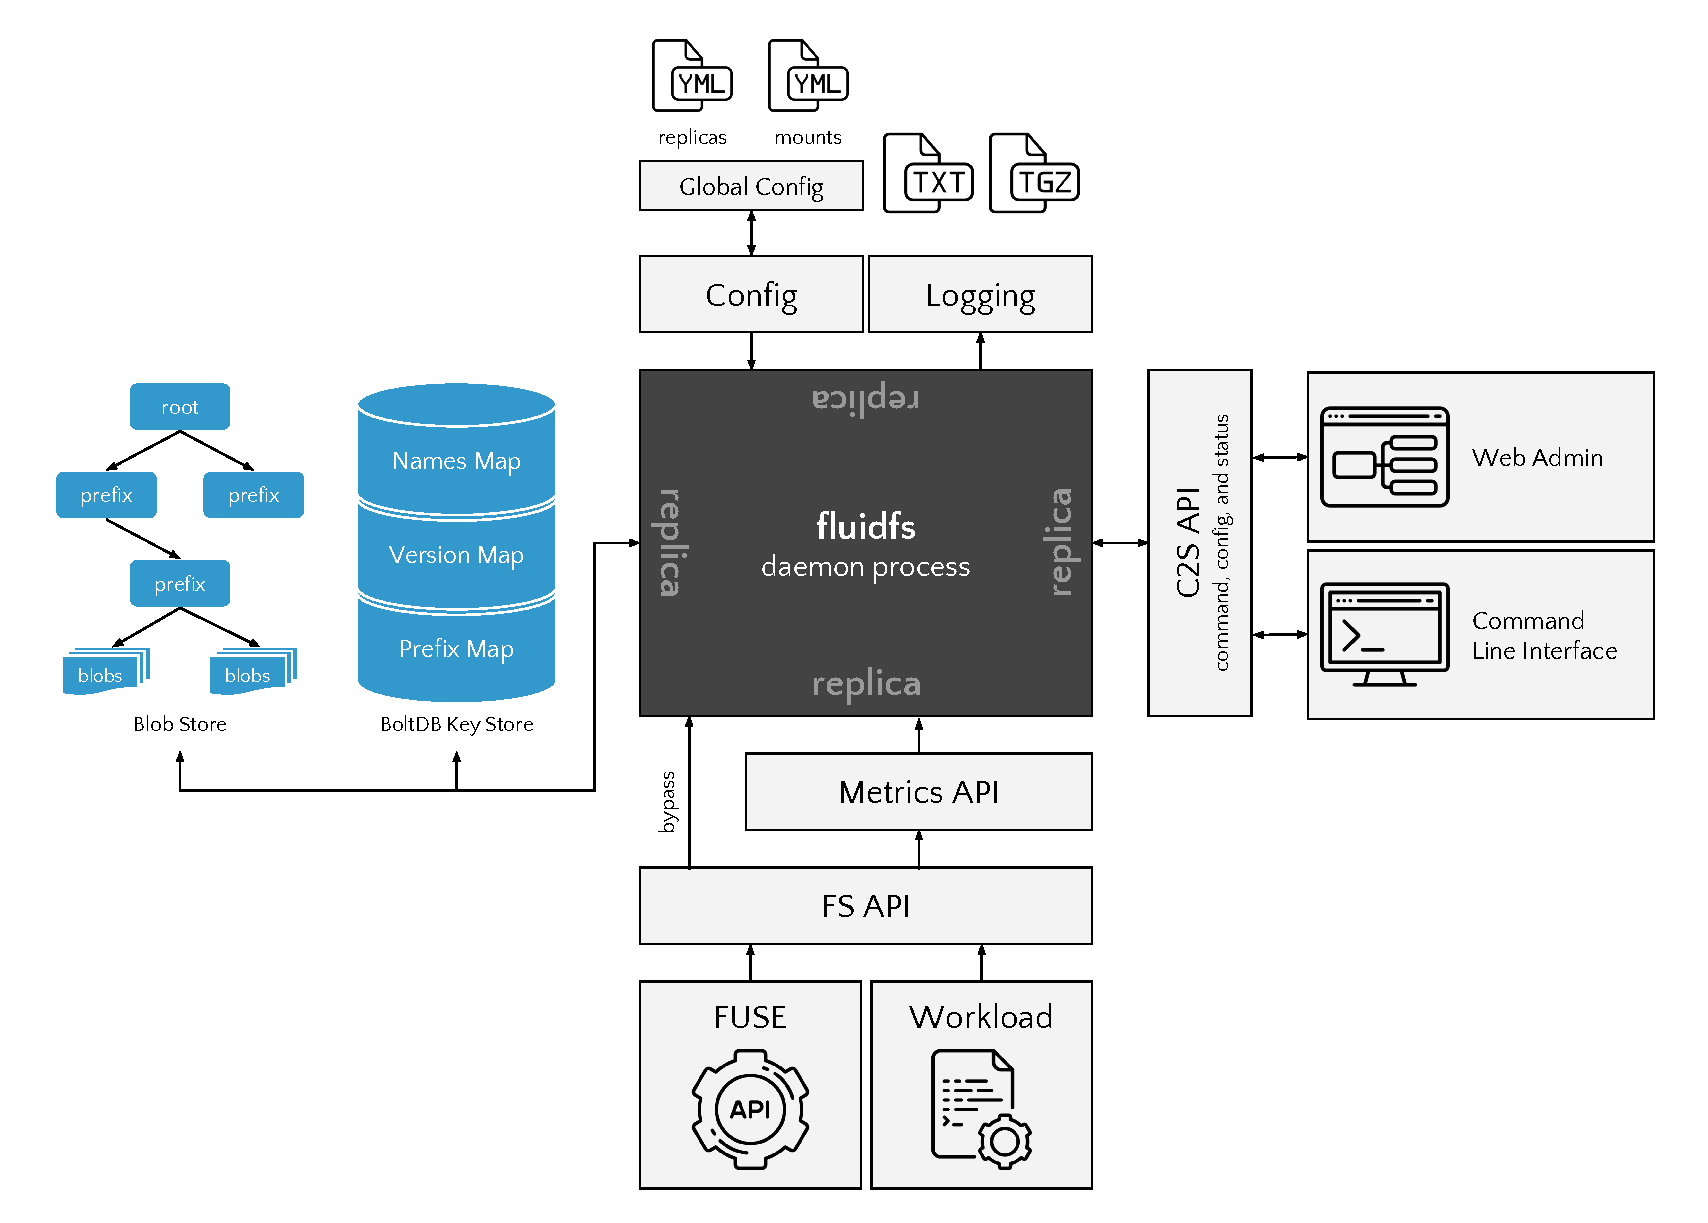
\includegraphics[width=\linewidth]{figures/ch05_fluidfs_replica.pdf}
    \end{center}
    \renewcommand{\baselinestretch}{1}
    \small\normalsize

    \begin{quote}
        \caption[FluidFS Architecture]{FluidFS implements the application component model specifically for a file system. Users interact with a local replica that implements the FUSE API or more directly through a gRPC API. The FluidFS daemon process stores data in a blob store and meta data in an embedded key/value store. The process also provides configuration and logging as well as a web interface for command and control.}
        \label{fig:ch05_fluidfs_replica}
    \end{quote}
\end{figure}
\renewcommand{\baselinestretch}{2}
\small\normalsize

The FluidFS replica architecture is specified in Figure~\ref{fig:ch05_fluidfs_replica}.
We have implemented two file system APIs, the first uses FUSE to implement a traditional POSIX-like interface by mounting a replicated volume to a local replica.
The second implements a client-server API to allow our file system to be accessible from mobile devices or sensors.
We also use the client-server API to perform benchmark and workload testing, avoiding the overhead of FUSE.
Each FluidFS replica maintains two primary data stores: a blob store on disk and an embedded key value store.
The embedded key value store must maintain three buckets: a mapping of names to version, a mapping of version to meta-data recipe, and mapping of object prefixes to location on disks or to other subquorums.
All FluidFS replicas also provide a web interface for command and control, allowing a user to directly view the configuration and behavior of a local replica and tune local optimization behavior.


\section{Conclusion}
\label{ch05_conclusion}

In this chapter we have briefly described our systems implementations of the two primary consistency protocols described in this dissertation and outlined our target applications.
Our systems are developed with the actor model in order to simplify reasoning about distributed architectures and to avoid common synchronization traps that cause edge conditions that violate consistency expectations.
A planetary scale system is composed of individual replicas with independent disk, memory, and processing capability and which can communicate with all other replicas in the network.
We outlined two replica types: the Alia replica which participates in hierarchical consensus, and the Honu replica which enables high throughput writes with relaxed consistency.

We implemented these replicas and our applications using the Go programming language with gRPC and protocol buffers for communication.
All of our code is open source and available on GitHub.
We intend to continue to develop the applications described in this chapter and deploy a planetary scale system.
Furthermore we welcome collaboration and would invite anyone interested to contribute to our codebase.
